 \documentclass[c]{beamer}
%\documentclass{beamer}
\listfiles

\mode<presentation>
{
  %\usetheme[deutsch,titlepage0]{KIT}
\usetheme[deutsch]{KIT}
% \usetheme{KIT}

%%  \usefonttheme{structurebold}

  \setbeamercovered{transparent}

  \setbeamertemplate{enumerate items}[circle]
  %\setbeamertemplate{enumerate items}[ball]

}
\usepackage{babel}
\date{}
%\DateText

\newlength{\Ku}
\setlength{\Ku}{1.43375pt}

\usepackage[utf8]{inputenc}
\usepackage[TS1,T1]{fontenc}
\usepackage{array}
\usepackage{multicol}
\usepackage{lipsum}
\usepackage[]{algorithm2e}
\usepackage{amsmath}
\usepackage{color}

\usenavigationsymbols
%\usenavigationsymbols[sfHhdb]
%\usenavigationsymbols[sfhHb]

\subtitle{Algorithmen I SS 14}
\author[]{Lena Winter}

\AuthorTitleSep{\relax}

\institute[ITI]{Institut für Theoretische Informatik}

\TitleImage[width=\titleimagewd]{images/title}

\newlength{\tmplen}

\newcommand{\verysmall}{\fontsize{6pt}{8.6pt}\selectfont}

\title[Algorithmen I SS 14]{Tutorium 11}

\usepackage{alltt}

\TitleImage[width=\titleimagewd]{images/alch}
\definecolor{OliveGreen}{RGB}{85,107,47}

\begin{document}

\begin{frame}
  \maketitle
\end{frame}

\begin{frame}{Greedy Algorithmen}
	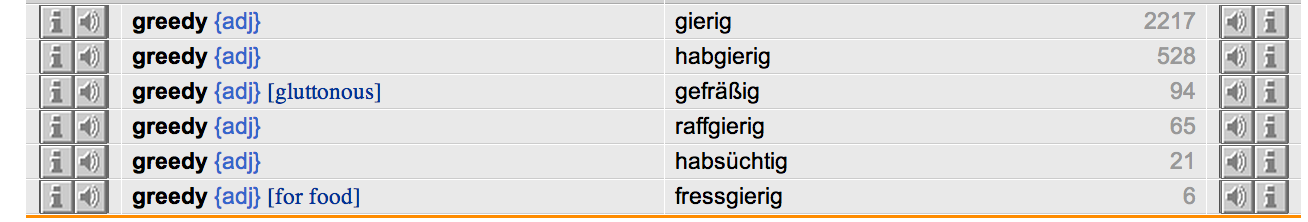
\includegraphics[width=\textwidth]{images/transla}
	\centerline{\huge{Idee}}
	\begin{itemize}
		\item Wähle für die \color{OliveGreen}aktuelle Situation\color{black} \ die optimale Entscheidung.
		\item Keine Reversion von vergangenen Entscheidungen
	\end{itemize}

\end{frame}


\begin{frame}{Eigenschaften}
	\begin{itemize}
		\item Global optimale Lösungen bestehen oft aus lokal optimalen Lösungen 
		\item Sinnvoll zum Annähern von Optima
		\item Einfach zu Implementieren
		\item Schnell
	\end{itemize}
	\includegraphics[scale = 0.2]{images/idee}

\end{frame}


\begin{frame}{Beispiele}
	\large{Greedy Algorithmen die optimale Ergebnisse liefern:}
	\begin{itemize}
		\item Dijkstra für Kürzeste Wege
		\item Beide MST Algorithmen
		\begin{itemize}
			\item Kruskal
			\item Jarnik-Prim
		\end{itemize}
		\item Selection Sort
	\end{itemize}

\end{frame}





\end{document}
